\documentclass[12pt]{article}

\usepackage{mathtools}
% \usepackage{graphicx}
\usepackage{parskip}
\usepackage[a4paper,margin=2.5cm]{geometry}
\usepackage{tikz}
% \usepackage{float}
% \usepackage{amssymb}
% \usepackage{subfig}
\usepackage[hidelinks]{hyperref}
\usepackage[citestyle=authoryear, style=authoryear, backend=biber]{biblatex}
% \usepackage{siunitx}
\addbibresource{manual.bib}
\usepackage{setspace}
\usepackage{enumitem}
\usetikzlibrary{3d,calc,intersections,patterns,positioning,tikzmark}

\raggedright
\linespread{1.3}
\setlist[description]{labelindent=1cm, leftmargin=!, labelwidth=1cm}

\renewcommand{\vec}[1]{\mathbf{#1}}

\author{Benjamin Williams \\ bmw@st-andrews.ac.uk}
\title{Manual for the \\ Magnetic Skeleton Analysis Tools Package \\ \( \; \) \\ Version 1.0}

\begin{document}

  \maketitle

  \tableofcontents

  \newpage

  \section{Introduction}

    The following manual describes the set-up of, and how to use, the Magnetic Skeleton Analysis Tools (MSAT) package that determine the magnetic skeleton of a 3D magnetic field \( \vec{B} \) (or any divergence-free vector field).

    The MSAT package consists of a null finder (which locates points where \( \vec{B} = \vec{0} \)), a sign finder (which also identifies the sign of each 3D null) and a separatrix surface finder (which identifies not only the separatrix surface of each null but at the same time all the separators linking the null points). Each of these codes will be described individually later in more detail.  All these codes can be run in cartesian, cylindrical and spherical coordinate systems, although running in cylindrical coordinates is currently untested.

    The null point finding package generally follows the null finding method described by \textcite{Haynes2007}, but a few changes. The spine, separatrix surface and separator finders also generally follow the basic ideas described in \textcite{Haynes2007}. The main differences and more details on the methods used in the codes can be found in \textcite{WilliamsPhD2018}.

    The MSAT package also includes codes to calculate the heliospheric current sheet and its curtains, as well as bald patches in global solar magnetic field data set that have spherical geometry.

    These codes that are written using the Fortran 2008 standard so should be compiler independent and are parallelised using OpenMP. They have been tested and compiled using the free-to-use GFortran 4.8.5 on Linux. It has also been provisionally tested to work well on Windows using the Windows Subsystem for Linux.

    The MSAT package also provides several scripts in Python and IDL for visualisation of the output which have been tested using recent versions of Python (3.5) and IDL (8.5). The Python visualisation tools should, in the main, work with Python 2, but as it will be officially unsupported in the near future, development has concentrated on Python 3.

    The following Python modules are used (and tested using the versions in brackets):
    \begin{enumerate}
      \item NumPy (1.12)
      \item Matplotlib (2.0)
      \item Mayavi (4.5) (some issues with python 3 currently using default package)
      \item igraph (0.7.1)
    \end{enumerate}

  \section{Quick Start for a Cartesian Data Set}

    \begin{enumerate}
      \item First you need to setup up your directories using the command
      
      \texttt{make setup data=/path/to/data/dir output=/path/to/output/dir}
      
      where
      \begin{itemize}
        \item \texttt{/path/to/data/dir} is the path to the directory where your 3D cube of magnetic data is stored. To see how to write your magnetic data in the correct format see Section~\ref{sec:prep_data}. 

        \item \texttt{/path/to/output/dir} is the path to the directory where the output files from the skeleton analysis of the data will be stored. This can be the same as your data directory.
      \end{itemize}

      \item Compile the Fortran MSAT packages.

      \texttt{make}

      \item Running the skeleton analysis codes in order: the null finder, then the sign finder and finally the separatrix surface and separator finder.

      In the commands below it is assumed that your data is saved in a file called \texttt{magfield.dat}.

      \texttt{./nf -i data/magfield.dat}

      \texttt{./sf -i data/magfield.dat}

      \texttt{./ssfxyz -i data/magfield.dat}

      \item Visualising the magnetic skeleton in python

      First you need to start python:

      \texttt{python}

      \texttt{import pyvis.model3d as m3d}

      \begin{itemize}
        \item To view the separatrix surfaces illustrated by a set of rings:
        \texttt{m3d.make(`data/magfield.dat', [`nulls', `separators', `spines', `sepsurf'])}
        \item To view the separatrix surfaces illustrated by field lines lying in them
        \texttt{m3d.make(`data/magfield.dat', [`nulls', `separators', `spines', `fanlines'])}
      \end{itemize}
    \end{enumerate}
    If any problems arise or for customisations please refer to the main part of the manual.

  \section{Set-up and Compilation using the Makefile}

    A makefile is provided to compile all the Fortran codes which do the main analysis of the data. First it is recommended that the directories for the data files and output from the codes be set up. The codes assume that all the original magnetic field data files are stored in a directory called \texttt{data} and all output is stored in \texttt{output} within the main directory of the codes.

    It is recommended the MSAT package of codes are stored in a different location to the magnetic field data that is analysed. For instance, the MSAT package could be stored in a home directory and the data on a local scratch disc. Symbolic links can then be used to redirect the input/output data storage areas of the codes. Then many copies of the codes do not need to be created and the codes can be relinked to wherever the analysis is required to be done.

    It is recommended symbolic links are created to link these files from the code directory to where the data is stored. This can be done using the command:

    \texttt{make setup data=/path/to/data/dir output=/path/to/output/dir}

    This will create the symbolic links called \texttt{data} and \texttt{output} linking to the specified directories \texttt{/path/to/data/dir} and \texttt{/path/to/output/dir} respectively and create a \texttt{mod} directory for the Fortran module files to be stored. This should be used to reset the locations of the symbolic links each time a new data set needs to be analysed. These two directories can be the same but we recommend having two separate directories.

    Issuing the command

    \texttt{make}

    will initiate compilation of all codes and create the compiled executables and by default will compile with OpenMP turned on.

    \subsection{Coordinate Systems}
      \label{sec:coord}

      The code has been written for cartesian, cylindrical and spherical coordinates. However, the only code that requires a difference due to coordinate system is the Separatrix Surface Finder. Three different versions are compiled:
      \begin{enumerate}
        \item \texttt{ssfxyz} - cartesian \( (x, y, z) \)
        \item \texttt{ssfrpz} - cylindrical \( (R, \phi, z) \)
        \item \texttt{ssfrtp} - spherical \( (r, \theta, \phi) \)
      \end{enumerate}
      so you just need to use the appropriate executable for your data.

    \subsection{Options}

      % The main option to change at compilation time is the coordinate system of the data. To switch coordinate systems, you specify the coordinate system at in the make command. To compile in spherical coordinates, for example, you type

      % \texttt{make coord=spherical}

      % Other options are \texttt{cartesian} (default if \texttt{coord} is not specified) and \texttt{cylindrical}.

      Debugging mode may be enabled if required. If this mode is chosen then more data is printed to the terminal during the running of all the analysis code and all optimisations by the compiler are turned off. This makes the codes run much slower due to printing, but also because the codes are optimised less. This should hopefully not be required, but if it is is should only be used on rare occasions by those who know what they are doing! It enables Fortran debuging options. This mode is enabled including the option \texttt{debug=on}.

      OpenMP may be turned off using \texttt{openmp=off}. It is on by default. The number of processors can be selected in the params.f90 file, Fortran will request the required number of processors on execution of the programs. See section \ref{sec:params} for details on selecting numbers of processors. Not all of the codes are parallelised. They may be parallelised in future.

  \section{Preparing the Data}
    \label{sec:prep_data}

    All the codes require a 3D divergence-free vector field, which from now onwards will be called a magnetic field. The codes also require the grid size of the data and corresponding coordinates of the grid points. The data must be stored in a binary unformatted data file and written in the following order:
    \begin{enumerate}
      \item Three 32-bit (long) integers, \( n_1 \), \( n_2 \) and \( n_3 \), containing the three dimension sizes of the grid.
      \item Three 64-bit (double precision) floating point \( n_1 \times n_2 \times n_3 \) arrays, e.g., \( B_1(n_1,n_2,n_3) \), \( B_2(n_1,n_2,n_3) \) and \( B_3(n_1,n_2,n_3) \), containing the magnetic field values at each grid coordinate.
      \item Three 64-bit (double precision) floating point 1D arrays, \( x_1(n_1) \), \( x_2(n_2) \) and \( x_3(n_3) \), containing the coordinates in each grid dimension.
    \end{enumerate}
    The 3D arrays must be written with Fortran order rather than C order. A Fortran ordered array of size \( n_1 \times n_2 \times n_3 \times 3 \) is equivalent to the three separate magnetic field arrays above.

    An example of creating a suitable data file in both IDL (Fortran order) and Python (C order) follows assuming the arrays are in their default memory orders for each language respectively. Assuming the magnetic field component arrays are stored as \texttt{bx}, \texttt{by} and \texttt{bz} of size \texttt{nx} by \texttt{ny} by \texttt{nz} and coordinate grids \texttt{x}, \texttt{y} and \texttt{z} with the correct bit sizes, you can save the data to file using:

    IDL:

    \begin{verbatim}
    openw, 10, `data/magfield.dat'
    writeu, 10, long([nx, ny, nz])
    writeu, 10, bx, by, bz
    writeu, 10, x, y, z
    close, 10
    \end{verbatim}
    Files are required to be stream files so there is no need to use the \texttt{/f77\_unformated} keyword in IDL when opening files. This allows all files to have random access.

    Python:

    \begin{verbatim}
    with open(`data/magfield.dat', `wb') as file:
        numpy.array([nx, ny, nz], dtype=numpy.int32).tofile(file)
        bx.T.tofile(file) # transpose is required
        by.T.tofile(file) # for memory order
        bz.T.tofile(file)
        x.tofile(file)
        y.tofile(file)
        z.tofile(file)
    \end{verbatim}

    Since Python uses C memory order, arrays must be transposed in NumPy to switch them to Fortran order for writing. There is also the option to create arrays in NumPy in Fortran order using the \texttt{order=`F'} keyword argument in the following NumPy command \texttt{array((nx, ny, nz), dtype=numpy.float64, order=`F')}. However I do not know whether this has the required effect when writing to file. NumPy's \texttt{meshgrid} function makes it easy to create grids from analytic functions -- see below in section \ref{sec:pythonanal} for more details and an example.

    An example of creating a suitable data file written using a Fortran code is given in \texttt{src/writedata.f90} (see Section~\ref{sec:writedata}). Note that the data file is written with stream access using the Fortran open keyword argument \texttt{access=`stream'} which allows the data files to be portable between languages.

    The equivalent data in spherical and cylindrical coordinates can be written to a file in the usual orders \( r \), \( \theta \), \( \phi \) in spherical and \( R \), \( \phi \), \( z \) in cylindrical coordinates. The grids in the angular directions must stretch over the whole angular domain i.e. \( 0 \) to \( 2\pi \) in \( \phi \) and \( 0 \) to \( \pi \) in \( \theta \). The codes will switch on periodic boundaries on the appropriate boundaries if spherical or cylindrical coordinates are turned on whether the angular directions are complete or not. Restricted angular domains may be available in future.

    \subsection{Creating a Data Set from an Analytical Expression in Fortran}
      \label{sec:writedata}

      The code \texttt{writedata.f90} allows you to create a data set from an analytical expression. It will be compiled at the same time as the main codes. To execute type

      \texttt{./writedata}.

      This will save a magnetic field (by default) as \texttt{data/magfield.dat}. To change the output file name type \texttt{writedata -o newfilename.dat} and the data file will be saved as \texttt{data/newfilename.dat}
    
    \subsection{Creating a Data Set from an Analytical Expression in Python}
      \label{sec:pythonanal}

      NumPy's \texttt{meshgrid} can be used which makes creating fields from an analytic expression very easy. But the option \texttt{indexing=`ij'} must be used otherwise the field will not be correct since the first two dimensions will be switched which is correct for plotting in Matplotlib.

      The following example writes a single null point magnetic field appropriately to file of the form
        \[ B_x = x + \frac{q - J_\parallel}{2} y \]
        \[ B_y = \frac{q + J_\parallel}{2} x + p y \]
        \[ B_z = J_\perp y - (p + 1) z \]
      with \( p = 1 \), \( q = 0 \), \( J_\parallel = 1 \) and \( J_\perp = 0 \) with grids from -1 to 1 using 200 points in each direction:

      \begin{verbatim}
    nx, ny, nz = 200, 200, 200
    xmin, xmax, ymin, ymax, zmin, zmax = -1, 1, -1, 1, -1, 1

    xgrid = numpy.linspace(xmin, xmax, nx, dtype=numpy.float64)
    ygrid = numpy.linspace(ymin, ymax, ny, dtype=numpy.float64)
    zgrid = numpy.linspace(zmin, zmax, nz, dtype=numpy.float64)
    x, y, z = numpy.meshgrid(xgrid, ygrid, zgrid, indexing=`ij')

    p, q, jpar, jperp = 1, 0, 1, 0
    bx = x + (q - jpar)*y/2
    by = (q + jpar)*x/2 + p*y
    bz = jperp*y - (p + 1)*z

    with open(`data/magfield.dat', `wb') as datafile:
        numpy.array([nx, ny, nz], dtype=numpy.int32).tofile(datafile)
        bx.T.tofile(datafile)
        by.T.tofile(datafile)
        bz.T.tofile(datafile)
        xgrid.tofile(datafile)
        ygrid.tofile(datafile)
        zgrid.tofile(datafile)
      \end{verbatim}

    \subsection{Using data created using Lare3D in IDL}

      Magnetic fields from Lare3D can also be used but require a bit of conversion since all the magnetic field components need to be moved to the same locations (centres of the grid cells). The following IDL code will do this conversion:

      \begin{verbatim}
    d = getdata(0, /magnetic_field, /grid)
    nx = n_elements(d.x)
    ny = n_elements(d.y)
    nz = n_elements(d.z)
    bx = (d.bx[1:-1,*,*] + d.bx[0:-2,*,*])/2 ; magnetic field
    by = (d.by[*,1:-1,*] + d.by[*,0:-2,*])/2 ; components now
    bz = (d.bz[*,*,1:-1] + d.bz[*,*,0:-2])/2 ; at cell centres
    x = d.x & y = d.y & z = d.z
      \end{verbatim}

      These variables can now be written to file as above ready for analysis. For other grids, ensure all magnetic field components are in the same locations and they can be written to file in the same way.

  \section{The Main Codes}

    The analysis codes are the core of the MSAT package. The three main codes are the null finder \texttt{nf}, sign finder \texttt{sf} and separatrix surface finder \texttt{ssf}. Each are run using the following command (assuming the data file is called \texttt{magfield.dat})

    \texttt{./nf -i data/magfield.dat}

    \texttt{./sf -i data/magfield.dat}
    
    \texttt{./ssf*** -i data/magfield.dat} (replacing \texttt{***} for the appropriate coordinate system, see section \ref{sec:coord})

    They must be run in the above order or they will not work as the next code depends on output from the previous code. From now on, the manual will assume the magnetic field data file is called \texttt{magfield.dat}.

    \begin{enumerate}
      \item \texttt{nf} first finds the locations of the null points (points where all three components of \( \vec{B} = \vec{0} \)) and writes these to file.
      \item \texttt{sf} then uses these locations to look for the spine and fan vectors of each null point and can thus determine the sign of the nulls.
      \item \texttt{ssf} then uses the null locations and fan vectors to trace out separatrix surfaces for each null and identify all separators connecting null points. \texttt{ssf} also traces the spines using the same tracing algorithm and writes them to file.
    \end{enumerate}
    The three codes work in grid coordinates (a coordinate given between 1 and \( n_x \) in the \( x \) direction for example). The output from each is all in real coordinates (a coordinate in the original coordinate system) unless grid coordinates are also outputted.

    All options for these are in \texttt{params.f90} and are described here with their defaults.
    
    \subsection{Parameters}
      \label{sec:params}

      None of the parameters below should need to be changed, but they are discussed such that in the unlikely event that they do need to be changed it is clear what they are used for.
      
      \subsubsection{Global}
        \begin{description}
          \item [\texttt{nproc = 4}:] the number of processors used in OpenMP. Set to zero to use the environment variable OMP\_NUM\_THREADS. If OMP\_NUM\_THREADS is not set, OpenMP will attempt to use all available cores. This parameter will be ignored if OpenMP is turned off.
        \end{description}

      \subsubsection{Null Finder}
        \begin{description}
          \item [\texttt{zero = 1e-10\_np}:] what the code considers to be ``zero''. This is used in deciding whether the magnetic fields at the final null point locations are small enough. Also important in solving the bilinear equations.
          \item [\texttt{sig\_figs = 6}:] the accuracy in the significant figures to which the code finds the null point locations in grid coordinates. So \texttt{sig\_figs = 6} means it finds the null location to an accuracy of \( 10^{-6} \) of a grid cell.
        \end{description}

      \subsubsection{Sign Finder}
        \begin{description}
          \item [\texttt{rspherefact = 50.0\_np}:] specifies what multiple of \texttt{sig\_figs} is the radius that is used to create a sphere centred on the null point where the spine and fan vectors of the null point are calculated i.e., if \texttt{rspherefact = 50} and \texttt{sig\_figs = 6} then the radius of the sphere is  \( 50 \times 10^{-6} = 5\times 10^{-5} \) of a grid point. This may be worth changing only if the code is struggling with a known true null.
          \item [\texttt{nphi = 90}, \texttt{ntheta = 45}:] specify how many points in the \( \phi \) and \( \theta \) direction respectively are placed initially uniformly on the sphere around the null for determining the spine and fan vectors.
        \end{description}

      \subsubsection{Separatrix Surface Finder}
        The parameters below relate to the points placed in a ring on the separatrix surface about the null.
        \begin{description}
          \item [\texttt{nstart = 500}:] the number of field line start points forming the initial ring about the null. This number is also the minimum number of points \texttt{ssf} will try to maintain during the separatrix surface analysis.
          \item [\texttt{pointsmax = 100000}:] specifies the maximum number points (field lines) on a ring. The code will move onto the next null if this number of points on a ring is reached.
        \end{description}
        
        These parameters relate to the rings used to determine the separatrix surface location
        
        \begin{description}
          \item [\texttt{stepsize = 0.2}:] the distance in grid coordinates between each of the rings. This is equivalent to saying the magnetic field line through each point on a r     ing is traced a distance approximately equal to \texttt{stepsize = 0.2} in grid coordinates before the next ring is formed.
          \item [\texttt{ringsmax = 10000}:] the maximum number of rings (excluding the first) that \texttt{ssf} will use to analyse each null's separatrix surface. If this number of rings is reached then the code will move onto the next null. For large boxes, this may need to be increased. The code will be able trace fieldlines a maximum of approximately \texttt{stepsize} \( \times \) \texttt{ringsmax} grid points away from the nulls.
        \end{description}
        
        These parameters relate to the tracing of the field lines via the Runge-Kutta-Fehlberg integration scheme.
        \begin{description}
          \item [\texttt{tol}, \texttt{stepmin}:] These are RKF45 parameters that relate, respectively, to the tolerance to which a field line is traced and the minimum step distance used for iteration of the scheme.
        \end{description}

    \subsection{Output Files}

      After running \texttt{nf}, \texttt{sf} and \texttt{ssf}, the following files should be created and can be read in using routines provided and described in Section~\ref{sec:vis}. If not specified below, the coordinates written to file are real coordinates.
      \begin{description}
        \item [\texttt{output/magfield-nullpos.dat}:] the null point locations in both grid and real coordinates
        \item [\texttt{output/magfield-nulldata.dat}:] the sign and spine and fan vectors for each null point
        \item [\texttt{output/magfield-ringinfo.dat}:] the number of points on each of the rings for all of the nulls
        \item [\texttt{output/magfield-rings.dat}:] the coordinates of all the rings together with break point and associativity data
        \item [\texttt{output/magfield-connectivity.dat}:] the null numbers which the separators connect and the ring and point numbers of the final ring where the separator exists
        \item [\texttt{output/magfield-separators.dat}:] the coordinates of all separators
        \item [\texttt{output/magfield-spines.dat}:] the coordinates of all the spine lines
      \end{description}

    \subsection{Warnings and Errors}
      \subsubsection{Sign Finder}
        The Sign Finder has three warning codes about each null to be aware about.
        \begin{description}
          \item [1:] The null is likely to be a source or a sink -- there may be an issue with the magnetic field itself.
          \item [2:] The null's spine vector and vector normal to the fan plane are almost parallel.
          \item [3:] The code early on tries to make a guess on the sign of the null based on which of the points converge first. This will be flagged if the guess and the final sign do not agree -- perhaps worth checking the null.
        \end{description}
        Errors with individual nulls can be checked using \texttt{nullstruct.py}. See later for more details.
      
      \subsubsection{Separatrix Surface Finder}
        The Separatrix Surface Finder will stop under the following circumstances:
        \begin{enumerate}
          \item a trace error occurs
        \end{enumerate}

  \section{Heliospheric Current Sheet (hcs) and Bald Patches (bp)}

    To be finished...

  \section{The code: \texttt{makecut}}

    Creates slices through the magnetic skeleton features to aid visualisation.

    Currently can only take cuts for a plane of constant \( x \)

    To be finished...

  \section{Visualisation routines}
    \label{sec:vis}

    Visualisation routines are available written in IDL and Python. These can be found in the \texttt{idlvis} and \texttt{pyvis} directories, respectively. For now, only the python routines are described. There are generally equivalent routines that do the equivalent operation in IDL as well.

    \subsection{Data Reading Routines}

      In \texttt{read.py}, there are routines for reading in all the output from the Fortran codes.

      The following command will be assumed for how the module has been imported:
      \texttt{import pyvis.read as rd}

      Below each of the python codes is described, as well as the command to use it. All the python codes require the filename as input, then there are additional options available to configure the output.

      \texttt{rd.nulls(`data/magfield.dat', simple=False)}

      \begin{description}
        \item [Description:] This code reads in the output from both \texttt{nf} and \texttt{sf}.
        \item [Option: \texttt{simple=False}:] If this option is set to \texttt{True} then only the null point locations are read in. This is useful if \texttt{sf} has not yet been run.
        \item [Returns:] A record array containing a dictionary like structure for each null is returned. This contains for each null
        \begin{itemize}
          \item its position in both real and grid coordinates
          \item its spine and both fan vectors
          \item its sign
          \item a null number (in fortran numbering) to help uniquely identify each null.
        \end{itemize}
      \end{description}

      \texttt{rd.separators(`data/magfield.dat', lines=True, connectivity=True, hcs=False)}

      \begin{description}
        \item [Description:] This code reads in the separators and the nulls connected by each separator.
        \item [Option: \texttt{lines=True}:] This option determines whether the coordinates of the separator lines are outputted. To suppress them set \texttt{connectivity=False}.
        \item [Option: \texttt{connectivity=True}:] This option determines whether the unique numbers of the nulls connected by the separators are outputted. To suppress them set \texttt{connectivity=False}.
        \item [Option: \texttt{hcs=False}:] This option outputs the separators connected to the heliospheric current sheet instead if set to \texttt{True}.
        \item [Returns:] A set of lists depending on the options above. The list contains an entry for each null containing a list of the separators and/or connectivities.
      \end{description}

      \texttt{rd.spines(`data/magfield.dat')}

      \begin{description}
        \item [Description:] This reads the spines of each null.
        \item [Returns:] It returns a list containing entries for each null consisting of an array with identifying the points that trace out each spine.
      \end{description}

      \texttt{rd.rings(`data/magfield.dat', allinfo=False, nskip=1)}

      \begin{description}
        \item [Description:] This reads in all the rings calculated for the separatrix surfaces and information on where each ring breaks, if required.
        \item [Option: \texttt{allinfo=False}:] To return the break and association information in the same form as the rings set to \texttt{True}.
        \item [Option: \texttt{nskip=1}:] a parameter which determines how many rings are outputted. By default, it is set to 1 which will output all rings. \texttt{nskip=2} will output every other ring, for example.
        \item [Returns:] a list containing an entry for each null which list the locations of the points in all required rings.
      \end{description}

      \texttt{rd.field(`data/magfield.dat')}

      \begin{description}
        \item [Returns:] a 6-element tuple containing arrays of the three magnetic field components and arrays of the three grid coordinates in this order.
      \end{description}

    \subsection{3D Visualisation}

      \texttt{model3d.py} has been written using the Mayavi module to visualise the structure of the fields in 3D.

      First import the module using \texttt{import pyvis.model3d as m3d}.

      The main routine can then be run as using the following command

      \texttt{m3d.make(`data/magfield.dat', addlist, nulls=None, box=True, fieldlines=None, linecolor=(0,0,0), nskip=20, nullrad=1, nfanlines=40, nring=None)}

      \begin{description}
        \item [Required:] \texttt{filename} and \texttt{addlist}.
        \item [Option: \texttt{addlist}:] should be a list of strings with the magnetic structures you wish to plot e.g. \texttt{[`nulls', `separators', `spines', `sepsurf']}. The other available option is \texttt{`fanlines'} which should used instead of \texttt{`sepsurf'} if preferred.
        \item [Option: \texttt{nulls=None}:] if this is set to \texttt{None} then all nulls will be plotted. Otherwise provide a list of specific nulls to plot, e.g. \texttt{nulls=[2, 3, 6, 9]} or \texttt{nulls=list(range(10, 20, 2))} only plots the null with those unique numbers (in Fortran numbering). Note, this also determines which spines and separators are also plotted.
        \item [Option: \texttt{box=True}:] set this to \texttt{False} to turn off the plotting of the outer box.
        \item [Option: \texttt{fieldlines=None}:] set this to a \texttt{(n, 3)} array to plot field lines passing through the list of specified points.
        \item [Option: \texttt{linecolor=(1,1,1)}:] set this to the RGB colour required for the fieldlines. e.g., \texttt{linecolor=(0,0,0)} is black (default),  \texttt{linecolor=(1,0,0)} is red, \texttt{linecolor=(0,1,0)} is green and \texttt{linecolor=(0,0,1)} is blue.
        \item [Option: \texttt{nskip=20}:] reduces the number of rings plotted. Choose how many rings to skip in when plotting the separatrix surfaces -- similar to \texttt{nskip} in the rings reading procedure. This will also determines the resolution of the spine and separator lines.
        \item [Option: \texttt{nullrad=1}:] set to reduce (if $<1$) or enlarge (if $>1$) the radius of the spheres used to identify the null points. The factor multiplies the default radius. The default radius is calculated based on the box size and grid spacing.
        \item [Option: \texttt{nfanlines=40}:] set this to the number of approximately equally spaced field lines drawn to map out the separatrix surfaces.
        \item [Option: \texttt{nring=None}:] the ring number (given the ring skipping value above) from which the fan field lines are drawn from. If \texttt{None} then the code will pick the ring a 5th of the way from the null.
      \end{description}

      This procedure will plot and open the window for viewing. The plot can be rotated using a left click-and-drag, zoomed by rotating middle mouse wheel and panned by a click-and-drag using the middle mouse wheel.

      This viewer is currently only implemented in cartesian coordinates. It will plot a spherical coordinate magnetic skeleton for example taking into account the periodic boundaries but it will be as if the three coordinates were cartesian. Also any calculated fieldlines will be done using a cartesian fieldline tracer and so will be incorrect.

      It is possible to add more magnetic skeleton features after the initial draw. There is an individual function for drawing each part of the magnetic skeleton which can be called separately. This is especially useful for drawing different sets of fieldlines individually. However the initial \texttt{make} must have been called. This will at least read in the required initial data. If you do not want anything to plot initally, set \texttt{addlist} to be an empty list.

      The following command will plot fieldlines from the \texttt{(n, 3)} array of points given in \texttt{startpts}
      
      \texttt{m3d.add\_fieldlines(startpts, col=(0,0,0), colquant=None)}.

      If \texttt{colquant} is given as a scalar array of the same size as the grid, the fieldlines will be coloured to vary with the quantity given in \texttt{colquant} and \texttt{col} will be ignored. Custom colormaps will be soon be added.

      For more documentation, such as how to save the plots drawn, see the Mayavi online documentation at \texttt{http://docs.enthought.com/mayavi/mayavi/mlab.html}. Once the plotting window is open, standard Mayavi commands can be used. The Mayavi module is imported inder the name \texttt{ml} in the \texttt{model3d} module or it can be imported into the main namespace.

      \subsection{Examples}

      Here are listed some examples of the indexing of the output from the data reading routines as the lists of lists etc. may become confusing.

      If the separators are read in using
      
      \texttt{seps, cons = rd.separators(`data/magfield.dat')}
      
      then the following indexing occurs:

      \begin{center}
        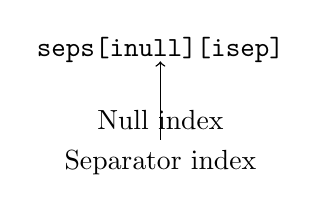
\begin{tikzpicture}[remember picture]
          \node at (0,0) {\texttt{seps[\tikzmark{inull1}inull\tikzmark{inull2}][\tikzmark{isep1}isep\tikzmark{isep2}]}};
          \coordinate (inull) at ($(pic cs:inull1)!1/2!(pic cs:inull2) - (0,1ex)$);
          \coordinate (isep) at ($(pic cs:isep1)!1/2!(pic cs:isep2) - (0,1ex)$);
          \draw[<-] (inull) -- ++(0,-0.5);
          \draw[<-] (isep) -- ++(0,-1);
          \node[below] at ($(inull) + (0,-0.5)$) {Null index};
          \node[below] at ($(isep) + (0,-1)$) {Separator index};
        \end{tikzpicture}
      \end{center}

      This will give an array of the coordinates of the \texttt{isep}\textsuperscript{th} separator from the \texttt{inull}\textsuperscript{th} null point.

      TBC...

  \printbibliography

\end{document}
